\section{Hastighedsmåler}


\subsection{Komponenter}
% Diode
% 555 timer
% Modtager diode

\subsection{Teori}



\subsection{Beregninger}
\subsubsection{555 timer modstande}
For 555 gælder det at vi ønsker en frekvens på 
\[
	f_{target} =  \SI{1000}{\hertz}
\]
\todo{Hvad var grunden til denne frekvens?}
Dette ønskes fordi at vores diode kan maksimalt klare en frekvens på.

Der kan opstilles 4 ligninger for 555 timeren således: 
For mark-time gælder det at
\begin{align}
	T_m &= 0.7 \cdot C_1 \cdot (R_1 + R_2) \label{eq:marktime} \\
\end{align}
For space-time gælder det at 
\begin{align}
	T_s &= 0.7 \cdot C_1 \cdot (R_2) \label{eq:spacetime} \\
\end{align}
For perioden gælder det at 

\begin{align}
	T &= \frac{1}{f} = T_s + T_m \label{eq:periodtime} \\
\end{align}
Og da dutycyclen skal være så tæt på $100$ som muligt sættes følgende forhold til at gælde
\begin{align}
	T_m &= 100 \cdot  T_s \label{eq:dutycycle} \\
\end{align}
Ved at løse ligningssystemet for ligningerne \ref{eq:spacetime}, \ref{eq:dutycycle}, \ref{eq:marktime}, \ref{eq:periodtime}, og isolerer for $R_1$ og $R_2$ og opskriver den som funktion af kapacitoren og frekvensen fås udtrykkende:
\begin{align}
	R_{1} \left( C_1,f \right) &= 1.400282885\,{\frac {1}{f \cdot C_1}} \\[2ex]
	R_{2} \left( C_1,f \right) &= 0.01414427157\,{\frac {1}{f \cdot C_1}}
\end{align}
Så antages at kondensatoren er 
\[
	C_1 = \SI{1.0d-6}{\farad}
\]
Da det antages vi bare benytter standardværdien. \todo{Er det standardværdien?***}

Frekvensen er nævnt og således bliver modstandende
\begin{align}
	R_1(\SI{1.0d-6}{\farad},\SI{1000}{\hertz})&= \SI{1400}{\ohm} \\[1ex]
	R_2(\SI{1.0d-6}{\farad},\SI{1000}{\hertz})&= \SI{14.14}{\ohm}
\end{align}

\subsubsection{Bestemmelse af modstande for peak-detektoren}

Vi har besluttet at benytte en peak-detektor til at opfange IR signalet til modtageren. Heraf benyttes der en simpel peak-detektor opbygning\todo{Er det den rigtige betegnelse***}.  Udtryk og teori benyttet er fra kilde \cite{peakdetectorCalc}.

Ud fra diodens karakteristika fås en forward-biased resistans på
\[
	r_{df} = \SI{607}{\ohm}
\]
og en reversed bias resistens på
\[
	r_{dr} = \SI{2d7}{\ohm}
\]
Således gælder det at vi skal vælge en modstand $R$ hvor det gælder at
\[
	r_{df} < R < r_{dr}
\]
Vores tidsvariable \todo{Rigtig betegnelse?} $\tau_2$ kan defineres som
\[
	\tau_2 = R \cdot C
\]
hvor $C$ er kapacitoren vi benytter i peakdetektoren.

\subsection{Test}
\todo{Der skal nok referes til billeder og navne på komponenter i billedet når der snakkes om tests***} 
\subsubsection{Afsender dioden}
Vi testede 555-timeren med et PC-oscilloskop.

På Figur ~\ref{fig:555noninv} er der en graf af den 555-timerens output, som det fremgår på info-boksene er duty cyclen er høj som beregnet. Det bemærkes også at frekvensen er lidt større end $\SI{1000}{Hz}$ men vi forventer ikke det giver os problemer.

Det inverterede signal kan ses på \ref{fig:555inv} og det fungerer som ønsket.
\begin{figure}[H]
	\centering
    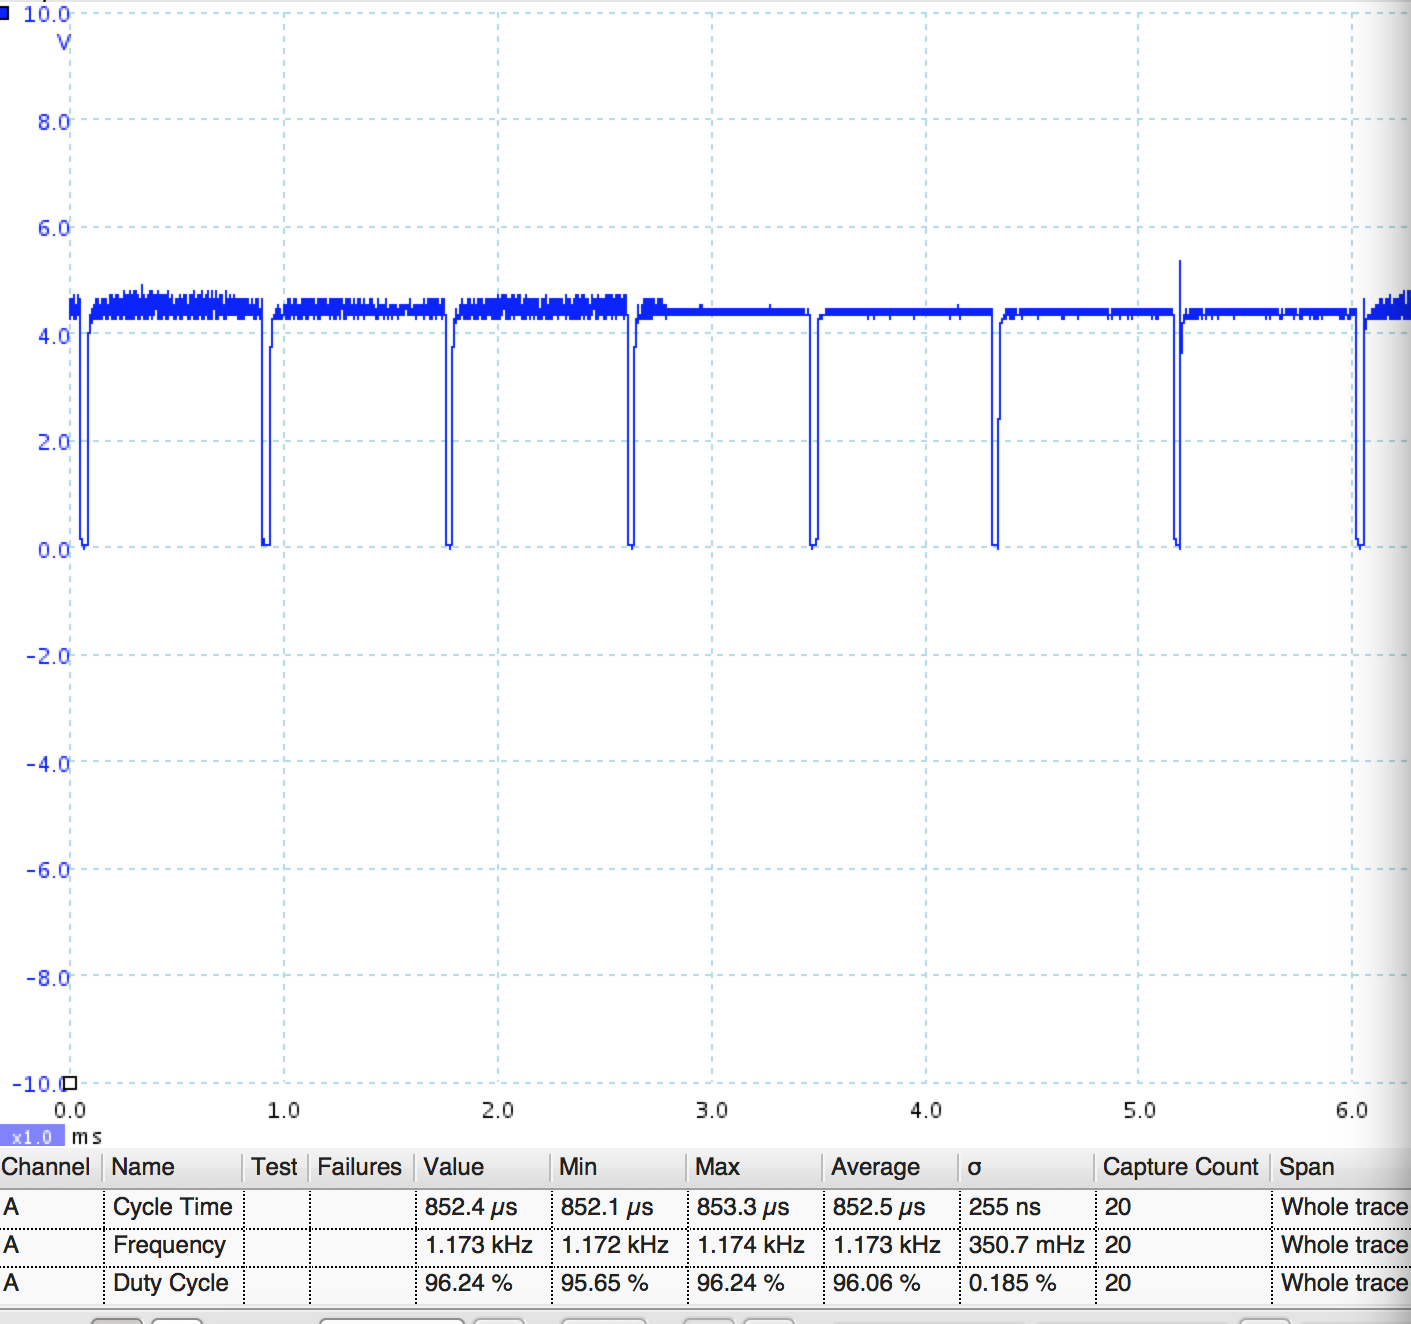
\includegraphics[width=13cm]{figures/2_4_3hastighed/555signal.png}
	\caption{Spænding som funktion af tiden med info-bokse i bunden}
	\label{fig:555noninv}
\end{figure}

\begin{figure}[H]
	\centering
    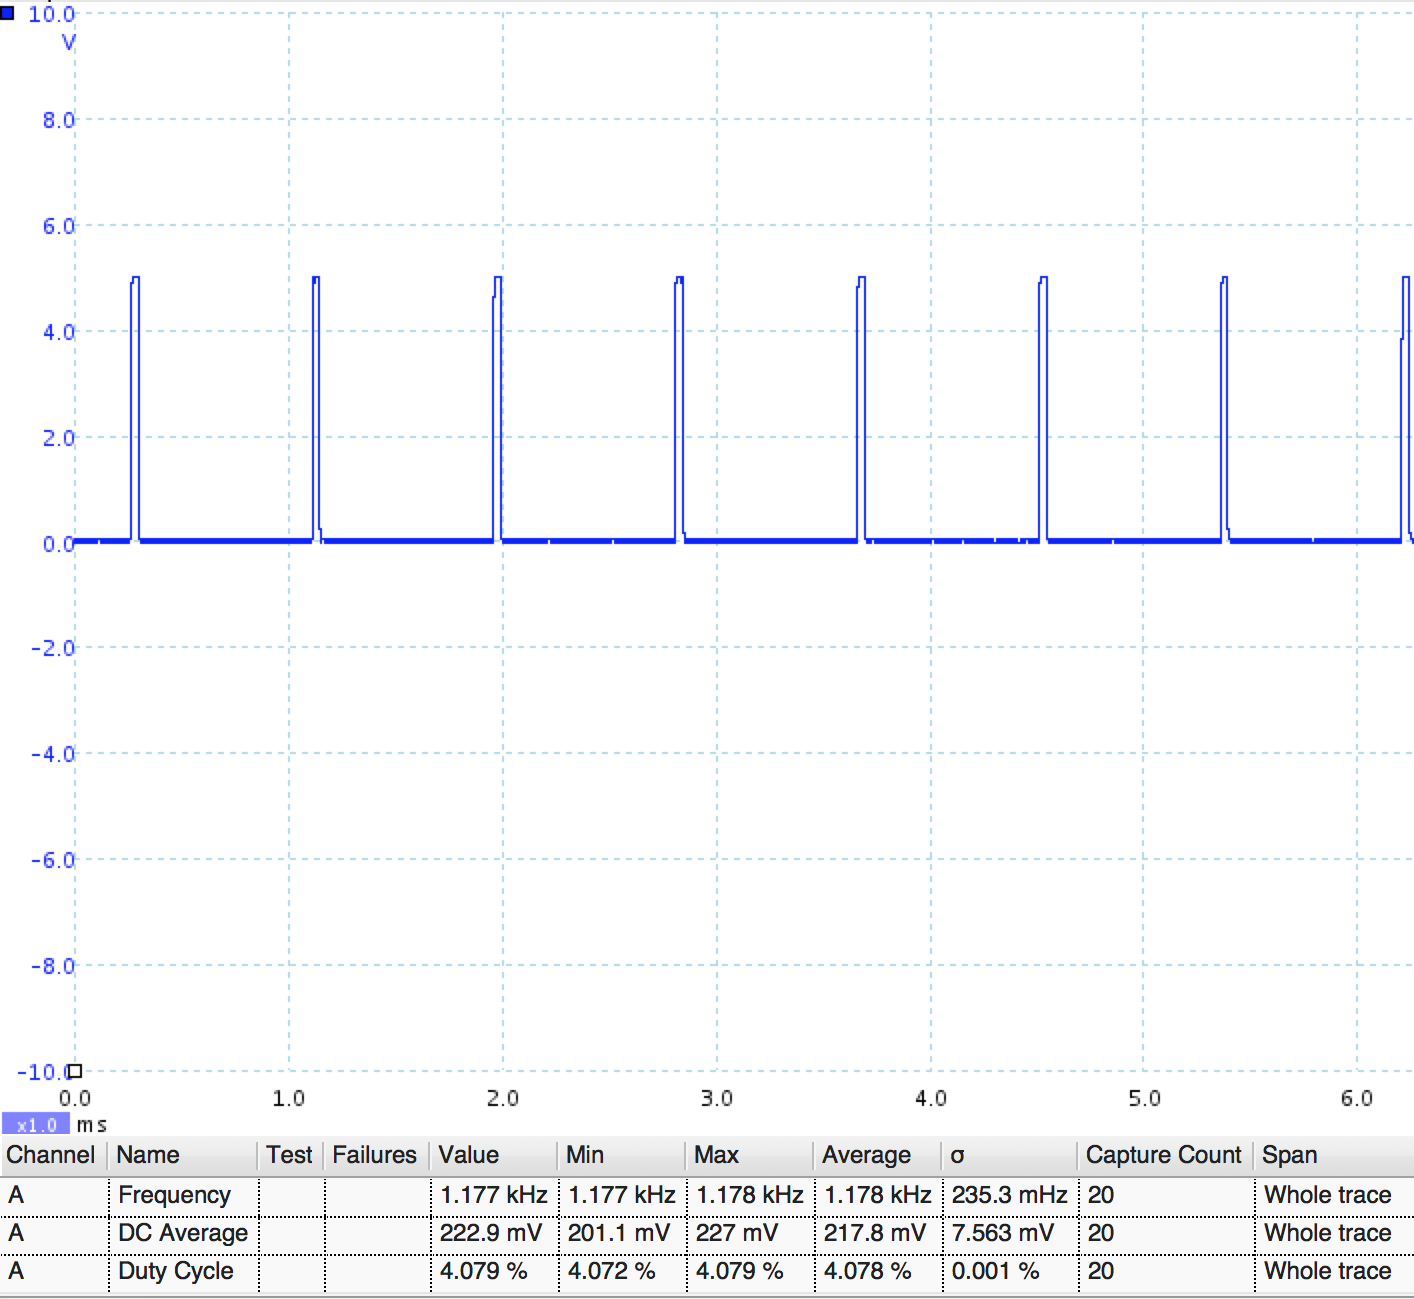
\includegraphics[width=13cm]{figures/2_4_3hastighed/555signalinv.png}
	\caption{Det inverterede signal som funktion af tiden med info-bokse i bunden}
	\label{fig:555inv}
\end{figure}

\begin{figure}[H]
	\centering
    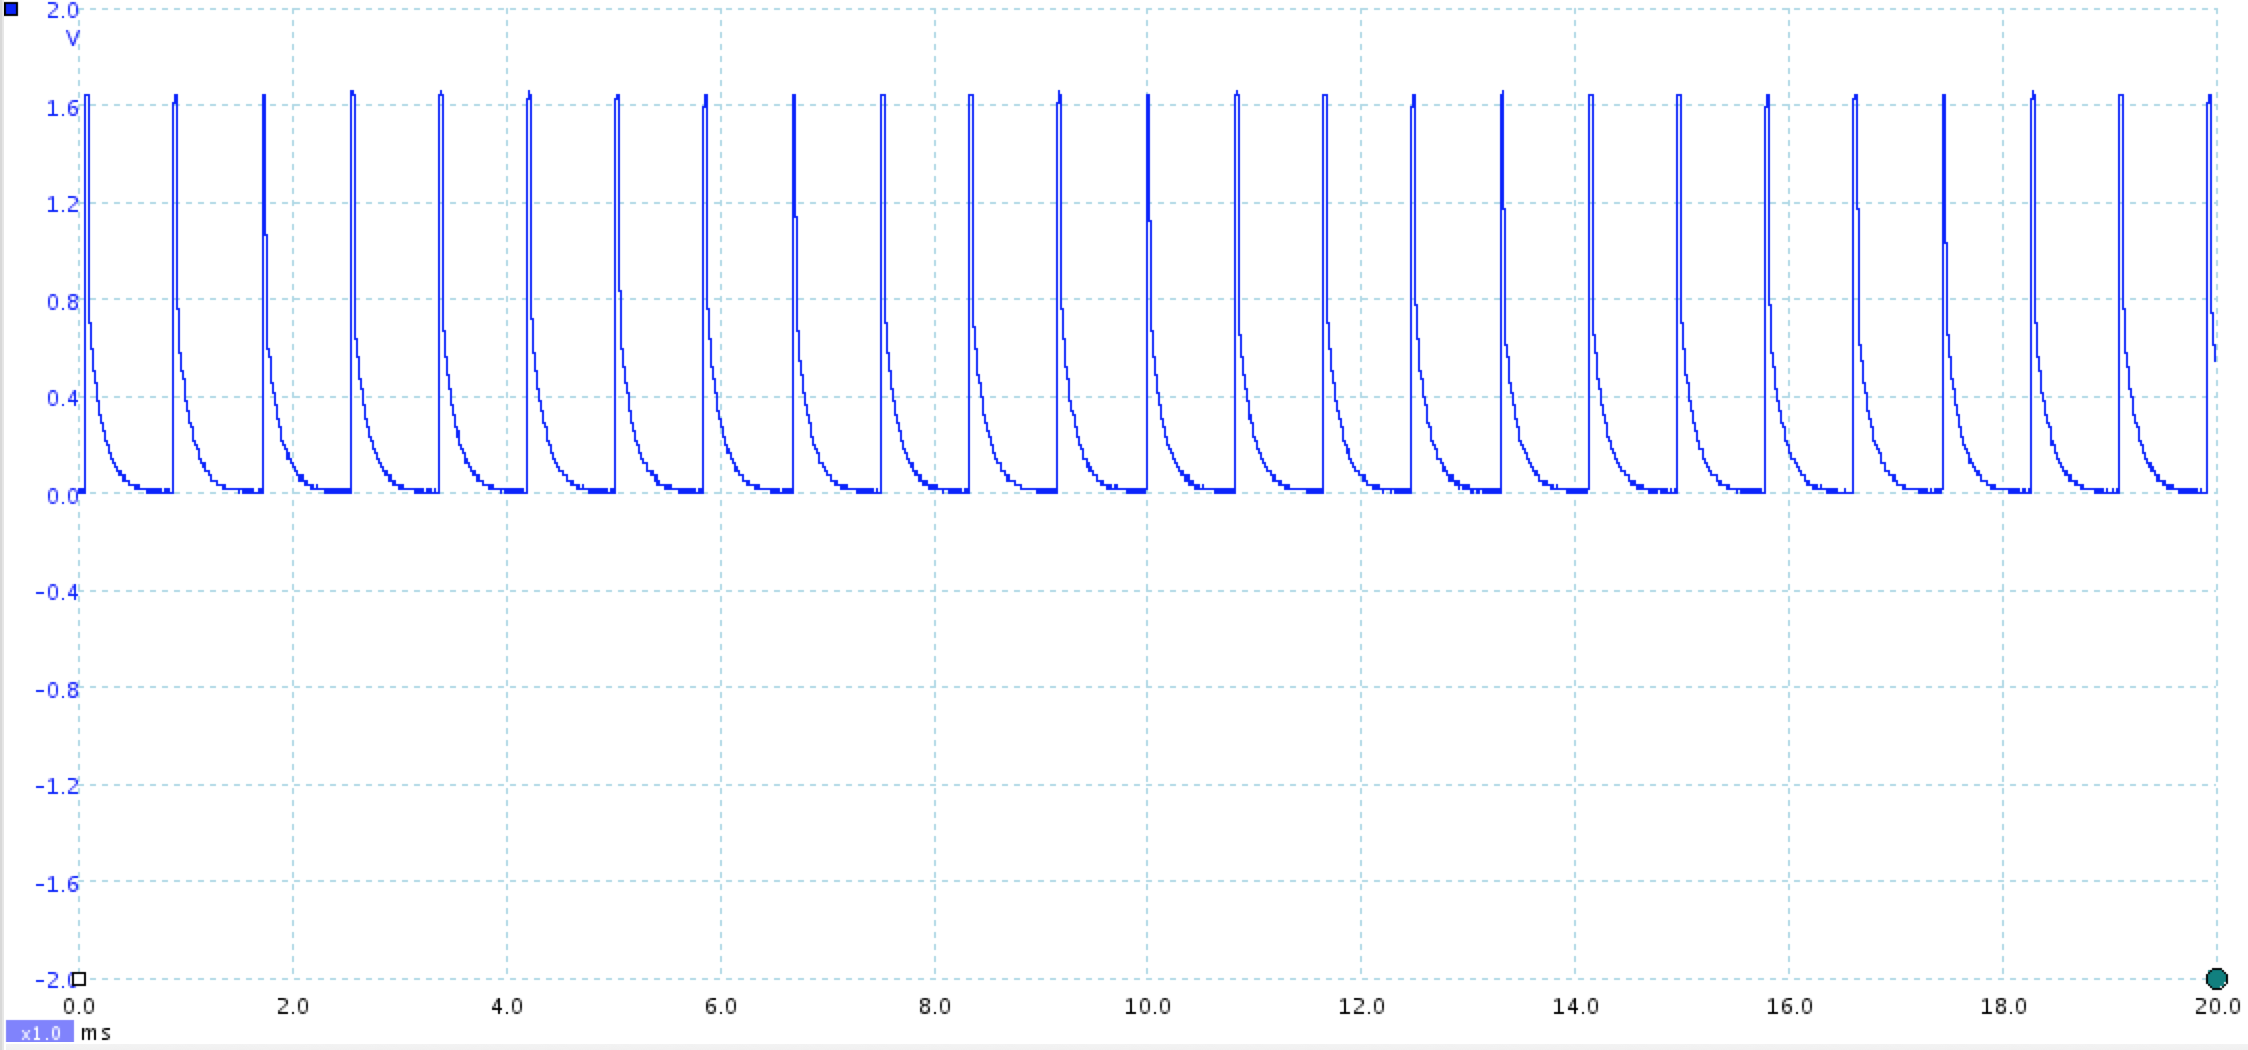
\includegraphics[width=13cm]{figures/2_4_3hastighed/555timerDiode.png}
	\caption{Spænding over dioden som funktion af tiden}
	\label{fig:diodeafsender}
\end{figure}
% 12/(10*10^(-3))
Spændingen over dioden kan ses på Figur ~\ref{fig:diodeafsender}.
Frekvensen estimeres ud fra de 12 første bølgetoppe. Heraf bemærkes at 

\[
	f_{diode} \approx \frac{12}{\SI{10d3}{s}} = \SI{1200}{Hz}
\]
Hvilket svarer fint til frekvensen af outputtet fra 555-timeren.

\subsubsection{Modtager dioden}
For modtager-delen af kredsen fremgår det på \ref{fig:IR_modtager} at frekvensen er omtrent $\SI{1.4d3}{Hz}$, og et tydelig spændingsforskel på omtrent $-\SI{5}{V}$ hvilket er et fint og tydeligt signal.
\todo{vi kunne muligvis godt have mere tekst her}
\begin{figure}[H]
	\centering
    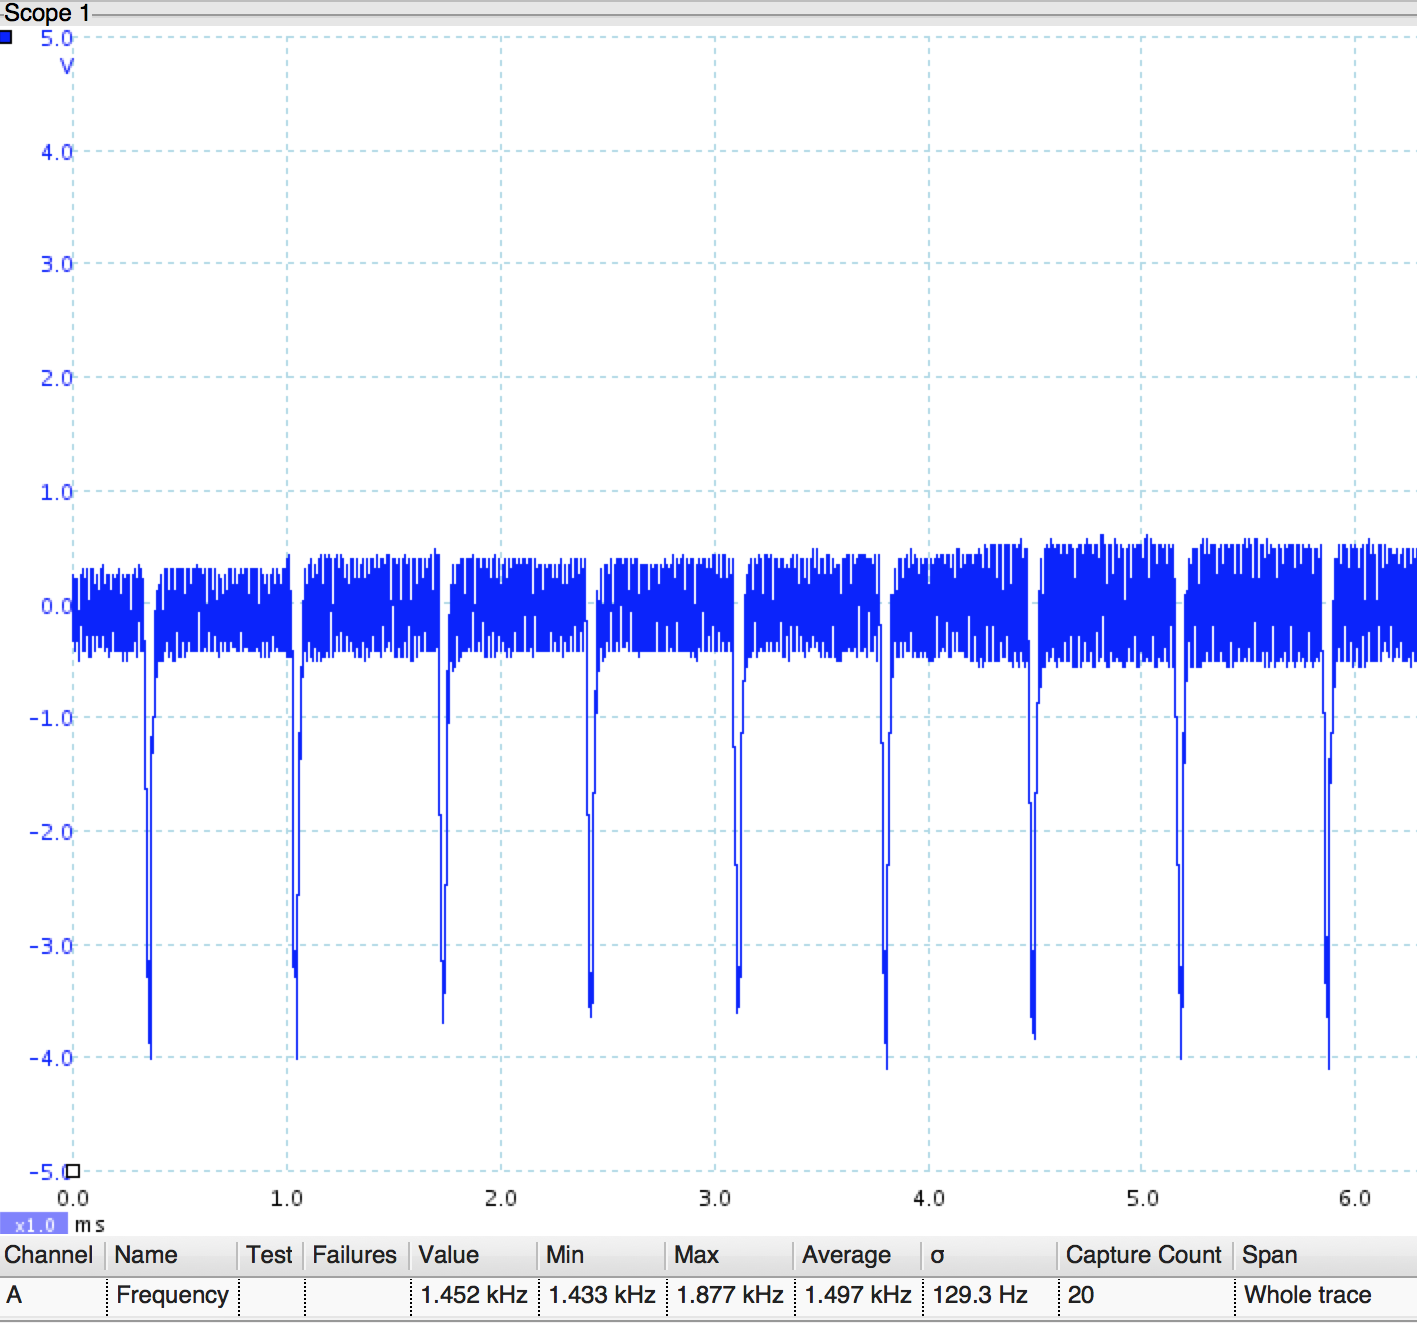
\includegraphics[width=13cm]{figures/2_4_3hastighed/IR_modtager.png}
	\caption{Spændingen som funktion af tiden af modtagerkredsens signal}
	\label{fig:IR_modtager}
\end{figure}

















